\documentclass[12pt, a4paper, openany, twoside]{book}
\usepackage[italian]{babel}
\usepackage[T1]{fontenc}
\usepackage[utf8]{inputenc}
\usepackage{amsmath} 
\usepackage{xcolor}
\usepackage[margin=1in]{geometry}
\usepackage{hyperref}
\usepackage{graphicx}
\graphicspath{{./img/}}
\usepackage{tikz}
\hypersetup{
    colorlinks=true,
    linkcolor=blue,
    filecolor=magenta,      
    urlcolor=cyan,
}
%usepackage[latin1]{inputenc}
\begin{document}
\fontfamily{cmss}\selectfont
\pagestyle{plain}
\author{DaveRhapsody}
\title {Analisi e Progettazione Software}
\date {30 Marzo 2020 (Sì, in ritardissimo, lo so)}
\maketitle
\tableofcontents
\chapter{Modelli di processo}
Per modello si intende una rappresentazione semplificata del processo, ed ognuno
di questi si basa su un aspetto specifico: 
\begin{itemize}
 	\item \textbf{Modello Workflow}
 	\item \textbf{Modello Data-Flow}
 	\item \textbf{Modello Role-Action}
 \end{itemize} 
 \paragraph{Modelli generici:}
 \begin{itemize}
 	\item \textbf{Modello a cascata:} A cascata significa che l'inizio dell'attività
 	successiva dipende dalla precedente, il che significa che se non è termminata
 	la precedente, non parte la successiva. 
 	\paragraph{Feedback:} Una volta arrivati al termine della cascata, si può
 	risalire a ritroso, sempre con la stessa regola, l'utente può fornire feedback
 	generalmente in seguito ai test del sistema (e vorrei vedere a consegnare
 	qualcosa di non testato).
 	\paragraph{Consegna incrementale:} Invece di rilasciare tutto il sistema di
 	botto alla fine, lo si rilascia in modo incrementale, poca roba per volta,
 	come alpha e beta nei videogiochi, stesso discorso. 
 	\subparagraph{Quali sono i vantaggi?} Alcune funzioni importanti sono disponibili
 	fin dal primo prototimo, hai meno rischi di fallimento, e i servizi a priorità
 	più alta sono collaudati più a fondo 	
 	\item \textbf{Modello ciclico:} Hai un certo numero di fasi, ciclicamente
 	le ripeti una dopo l'altra all'infinito, come una spirale.
 	\item \textbf{Ingegneria software basata sui componenti}
 \end{itemize}
Il concetto è che in base al modello, cambia completamente il modo in cui si
affronta lo sviluppo di un software, occorre (per trovare il migliore per le
proprie esigenze) capire quale modello usare, e quando.
\section{Modello UP (Unified Process) e RUP (Rational Unfied Process)}
E' un processo iterativo e incrementale, che suddivide un processo gigante in 
iterazioni più controllate. 
\paragraph{In sintesi:} Poca roba per volta, feedback più rapidi, iterazioni
di lunghezza definita e fissata, e modellazione con UML
\paragraph{Organizzazione del processo:}
\begin{enumerate}
	\item Avviamento
	\item Elaborazione
	\item Costruzione
	\item Transizione 
\end{enumerate}
Ogni ciclo è un incremento, e questo porta vantaggi legati a minori fallimenti,
riduzione precoce dei rischi, progrwssi più visibili, feedback precoci. 
Come caratteristiche principali ha che è iterativo e incrementale, ha maggiore enfasi
sul modello invece che sul linguaggio naturale, e si centra sull'architettura.\\
\section{Processo Scrum}
E' un processo iterativo che si basa sul controllo dello stato di avanzamento.
Come principi essenziali ha:
\begin{itemize}
	\item \textbf{Visibilità}: Gli aspetti significativi devono essere visibili
	per tutti
	\item \textbf{Ispezione}: Letteralmente si ispeziona frequentemente il lavoro
	per capire se si sta andando nella direzione giusta
	\item \textbf{Adattamento}: Se si sta deviando dagli obbiettivi servirà
	un adattamento per minimizzare le deviazioni
\end{itemize}
\subsection{Ruoli}
\begin{enumerate}
	\item \textbf{Product Owner}: Definisce le caratteristiche del progetto da 
	sviluppare (1 persona sola), e gestisce il Product Backlog
	\item \textbf{Team}: Dedicato allo sviluppo e rilascio del prodotto tramite
	incrementi successivi (da 3 fino a 8 membri)
	\item \textbf{ScrumMaster}: Responsabile del fatto che lo SCRUM venga applicato
	nel modo corretto
	\paragraph{NON E' UN PROJECT MANAGER:} Il PM gestisce il lavoro, lo SM invece
	soltanto il processo scrum, son due cose diverse. Inoltre lo SM riduce il Gap
	tra il PM e lo sviluppo, supporta il PM, facilità creatività e affiatamento
	del team, è praticamente un motivatore.
\end{enumerate}
\subsection{Catatteristiche}
\begin{enumerate}
	\item \textbf{Release brevi}: I sottoinsiemi vengono cosegnati presto
	\item \textbf{Progetto semplice}: In ogni istante tutti i test sono eseguibili,
	c'è un numero minimo di funzionalità e non hai logica duplicata
	\item \textbf{Refactoring}: Banalmente, rolling release, miglioramento continuo
	\item \textbf{Testing First}: Il testing è continuo
	\item \textbf{Pair programming}: Più sviluppatori lavorano insieme
	\item \textbf{Collective Ownership}: Il software non è di Pippo o Pluto, ma 
	del team composto da essi
	\item \textbf{Continuous integration}: Si hanno integrazioni continue e check-in
	frequenti
	\item \textbf{Cliente sul campo}: Nel senso che il cliente è rompicazzo e 
	lavora con il team.. Non so quanto positiva questa cosa, dipende da cliente
	a cliente.
\end{enumerate}
\chapter{Sistemi Socio-Tecnici}
\paragraph{Definizione di sistema:} E' un insieme di componenti che lavorano 
assieme per un obbiettivo comune
\begin{itemize}
	\item Può essere sw + hw, questa cosa è già vista in Reti e Sistemi Distribuiti
\end{itemize}
\section{Categorie di sistema}
\subsection{Tecnico-Informatici} Includono Hw + Sw e non includono operatori e 
processi operazionali. Inoltre il sistema non conosce lo scopo del suo utilizzo.
\subsection{Socio-Tecnici} Includono uno o più sistemi tecnici, ma anche i 
processi operazionali e gli operatori, però di contro sono condizionati dalle
politiche aziendali e dalle regole aziendali
\paragraph{Caratteristiche:}
\begin{enumerate}
	\item \textbf{Proprietà emergenti}:
	Le proprietà del sistema finale dipendono dalle sue componenti e dalle 
	relazioni tra le compoenti, possono essere misurate solamente sul sistema 
	finale
	\item \textbf{Non-Determinismo}: Il sistema non risponde sempre con lo stesso
	output dato lo stesso input perchè è indipendente dagli operatoi umani
	\item \textbf{Complesso legame tra i sistemi e gli obbiettivi aziendali}: 
	L'efficacia nel supportare gli obiettivi aziendali non dipende dal sistema stesso
	\paragraph{Esempi di proprietà emergenti:}
	\item Volume di un sistema (spazio occupato)
	\item Affidabilità
	\item Protezione
	\item Riparabilità
	\item Usabilità
	\paragraph{Proprietà del tipo "NON DEVE ACCADERE"}
	Prestazioni o affidabilità possono essere \underline{misurate}, ma altre proprietà
	consistono in cose che non devono succedere, dal punto di vista della
	\textbf{sicurezza} ma anche della \textbf{protezione}. 
\subsection{Organizzazione/Persone/Sistemi}
I sistemi socio-tecnici sono pensati per obbiettivi aziendali, o organizzativi,
nel senso che \textbf{se non si comprende l'ambiente organizzativo in cui un sistema è usato,
allora le probabilità che so sviluppiun sistema soddisfacente son basse}
\end{enumerate}
\subsection{Sistemi critici}
\begin{enumerate}
	\item \textbf{Sistemi safety-critical}: Un fallimento porta anche fino 
	alla morte di una vita umana	
	\item \textbf{Sistemi mission-critical}: Un fallimento ti manda all'aceto
	tutta l'attività a obbiettivi diretti (sistema di navigazione di un veicolo
	spaziale difettoso)
	\item \textbf{Sistemi business-critical}: Perdite di soldi
\end{enumerate}
\subsection{Tipi di fallimenti}
\begin{itemize}
	\item \textbf{Fallimento Hardware}: Errori di produzione o consumo
	\item \textbf{Fallimento Software}: Errori del programma
	\item \textbf{Errori operativi}: I classicissimi errori umani
\end{itemize}
\paragraph{Riporto dalle slides l'esempio del caso Mizuho Securities:}
\begin{center}
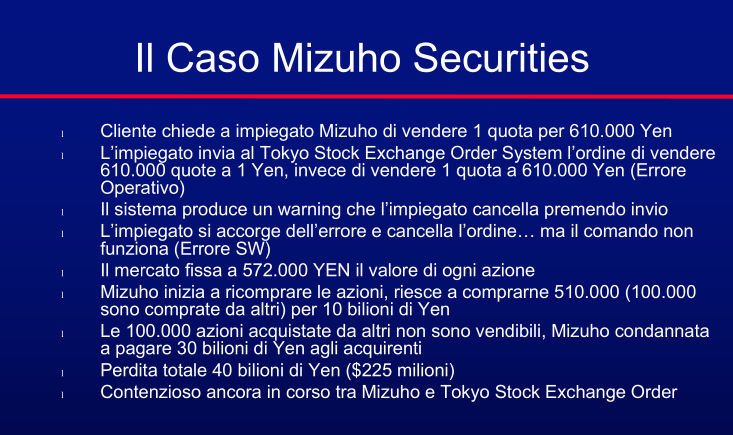
\includegraphics[width=0.75\textwidth]{1}
\end{center}
\subsection{Fidatezza dei sistemi}
Nei sistemi critici, generalmente la fidatezza è la più importante proprietà del
sistema, per via dell'alto costo di un fallimento.
\paragraph{Utilità e fidatezza non sono la stessa cosa:} Un sistema può essere utile
anche se gli utenti non hanno confidenza nel suo buon funzionamento.
\subsection{Altre proprietà}
\begin{enumerate}
	\item Riparabilità: Riflette la facilità con cui un sistema può essere 
	riparato in caso di errori
	\item Mantenibilità: Come si adatta il sistema a requisiti nuovi
	\item Sopravvivenza: Come fornisce servizi un sistema sotto attacco
	\item Tolleranza degli errori: quanto si tollerano errori di immissione?
\end{enumerate}
\subsection{Metodi di sviluppo per sistemi critici}
A causa del costo dei fallimenti, si hanno software di protezione che sono tutto
meno che economici, e questo è dato dal fatto: pensa quanto risparmi avendo più
sicurezza, confrontato a quanto perdi se un attacco va a buon fine, that's it.
\paragraph{Economie di fidatezza:} A causa del costo di un sistema dotato di 
elevata fidatezza, potrebbe essere conveniente sviluppare un sistema non fidato e
pagare per i costi di fallimento (Pagare con la vita dei propri operai, per esempio).
\begin{itemize}
	\item La scelta dipende da fattori politici e sociali, qui la concorrenza se
	per ipotesi il prezzo fosse davvero la morte di qualche operaio, vince a mani
	bas
	\item La scelta dipenderà dal sistema, per un normale sistema di business, una
	fidatezza moderata può essere sufficiente
\end{itemize}
\section{Analisi dei requisiti}
E' un processo di ricerca, analisi, documentazione e verifica dei servizi richiesti
dal cliente e i vincoli entro i quali i servizi devono operare
\subsection{Tipi di requisito}
\begin{enumerate}
	\item Requisito utente: Affermazioni in \textbf{Linguaggio naturale}, corredate
	da tabelle e diagrammi che riguardano i servizi che il sistema offre, al cliente
	glieli si dà scritti
	\item Requisito di Sistema: E' la base per il progetto della soluzione, può
	essere illustrato utilizzando i modelli di sistema 
	\item Requisito funzonale: E' l'insieme dei servizii che il sistema deve o non
	deve fornire
	\item Requisito NON-funzionale: REquisito del prodotto, requisito esterno o 
	anche organizzativo
	\begin{itemize}
		\item Prodotto: come deve comportarsi il prodotto
		\item Organizzativo: Politiche di organizzazione del cliente, se lavori 
		per RadioMaria, il sistema non bestemmia, per intenderci
		\item Esterno: Il sistema deve rispettare le norme di dove verrù usato.
		Tipo un drone deve rispettare le leggi dei droni, questo discorso.
	\end{itemize}
\end{enumerate}
\paragraph{Problemi dei requisiti}
\begin{enumerate}
	\item Ambiguità: Non è chiaro chi fa cosa
	\item Incompletezza: Non è possibile avere un documento dei requisiti completo
	\item Inconsistenza: Una descrizione non deve contenere contraddizioni o 
	conflitti.
	\paragraph{Esempio: } Avendo due requisiti di questo tipo:\\
	> l’utente riceve tutte le news pubblicate dal suo ultimo accesso\\
	> le news pubblicate rimangono disponibili per 7 giorni	 
\end{enumerate}
Siccome specificare i requisiti in linguaggio naturale fa schifissimo forever,
allora si usano alternative a quest'ultimo, come scrittura dei requisiti in un
formato standard, oppure ci si basa sullo standard IEEE 830
\section{Casi d'uso}
Documentano requisiti funzionali, complementari alla lista dei requisiti NON
funzionai, ed è il punto di partenza per analisi e progettazione. Ad esempio una
strada, potrebbe esser vuota o trafficata
\paragraph{Tipi di attore:} 
\begin{itemize}
	\item Attore primario, raggiunge degli obbiettivi utente utilizzando i
	servizi del sistema
	\item Attore di supporto, offre un servizio (tipo hosting web)
	\item Attore fuoriscena, ha interesse nel caso d'uso, ma non è attore nè
	primario nè supporto (Esempio, la struttura universitaria)
\end{itemize}
\paragraph{Formato breve:} E' un ottimo modo di prendere appunti rapidamente MA,
mancano scenari alternativi, (formato informale), e c'è una descrizione approssimativa.
\paragraph{casi d'uso informale:}
\begin{itemize}
	\item Scenario di successo principale: un cliente arriva alla cassa con della
	roba da restituire, il cassiere usa il pos per registrare ogni articolo
	restituito
	\item Scenari alternativi: Se il cliente aveva pagato con carta, e l'operazione
	di recesso è respinta, allora vene informato e rimborsato in contanti.
	\item Se il cliente rileva un fallimento nell comunicazione con il sistema
	esterno di gestione etc. etc.
\end{itemize}
\paragraph{Formato dettagliato:}
\begin{center}
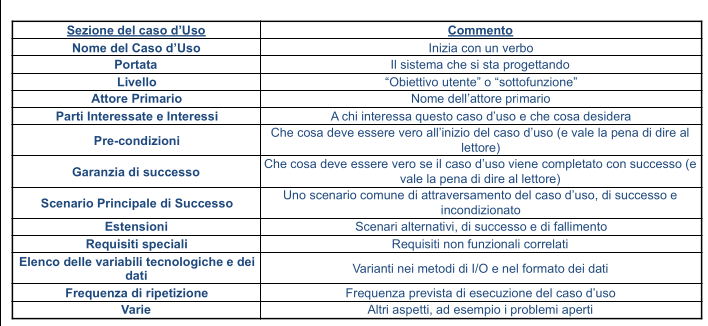
\includegraphics[width=0.75\textwidth]{2}
\end{center}
\subsection{Linee guida sulla scrittura dei casi d'uso}
Bisogna concentrarsi su qual è lo scopo dell'attore e cosa deve fare il sistema,
il come e l'interfaccia, per ora non ci riguardano, non ci interessano
\subsection{Test del capo}
Per capire differenza tra Caso d'uso e funzionalità, SE il capo chiede "cosa 
avete fatto", e gli rispondi con il nome del caso d'uso, sarà soddisfatto?
\subsection{Test EBP (Elemebtary Business Process)}
Attività che aggiunge un valore di business misurabile e lascia i dati in uno 
stato coerente
\subsection{Test della dimensione}
Ad una sola azione possono corrispondere da 3 a 10 pagine di specifiche nel formato
dettagliato.
\paragraph{Come si organizzano questi casi d'uso? Con i diagrammi dei casi d'uso}
\subparagraph{Esempio:}	
\begin{center}
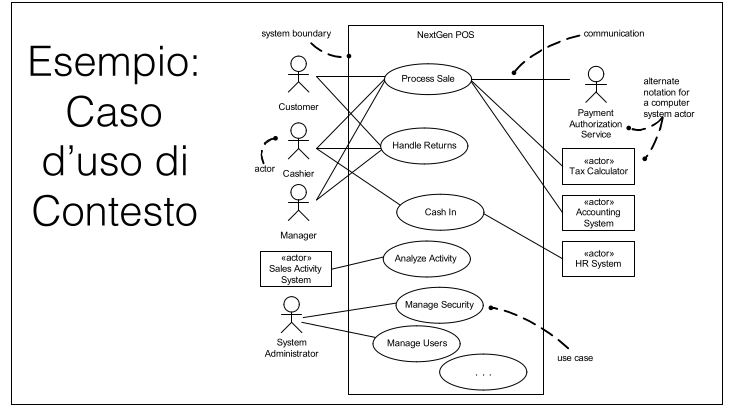
\includegraphics[width=0.75\textwidth]{3}
\end{center}
\paragraph{In breve:} Hai una serie di casi d'uso, una serie di attori e le
relazioni tra questi, i diagrammi sono secondari, il caso d'uso è un documento
di testo.
\paragraph{L'associazione} è un canale di comunicazione tra attore e caso d'uso,
si rappresenta con una line continua direzionata da chi dà inizio all'interazione
OPPURE anche non direzionata per intendere che entrambe le parti possono dare inizio.
\subsection{Tipi di relazione tra casi d'uso}
\begin{itemize}
	\item \textbf{Inclusione}:
	\begin{center}
	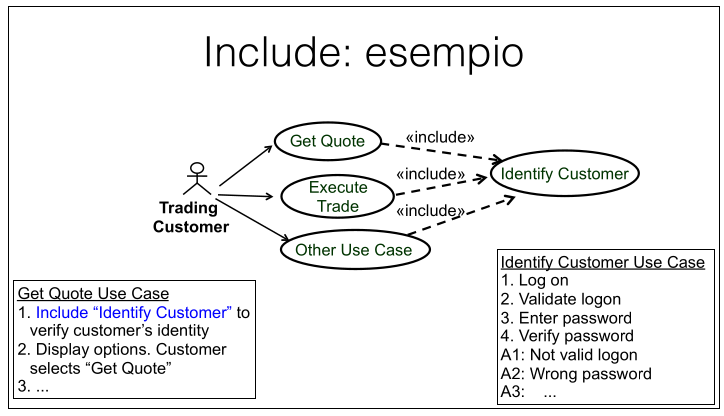
\includegraphics[width=0.75\textwidth]{4}
	\end{center}
	Lega un caso d'uso base ed uno incluso al suo interno
	\item \textbf{Estensione}:
	\begin{center}
	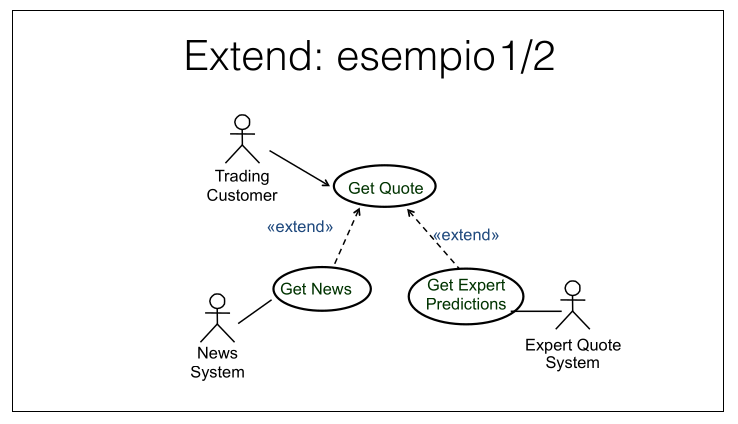
\includegraphics[width=0.75\textwidth]{5}
	\end{center}
	Connette ad un caso d'uso esteso un caso base
	\item \textbf{Generalizzazione}:
	\begin{center}
	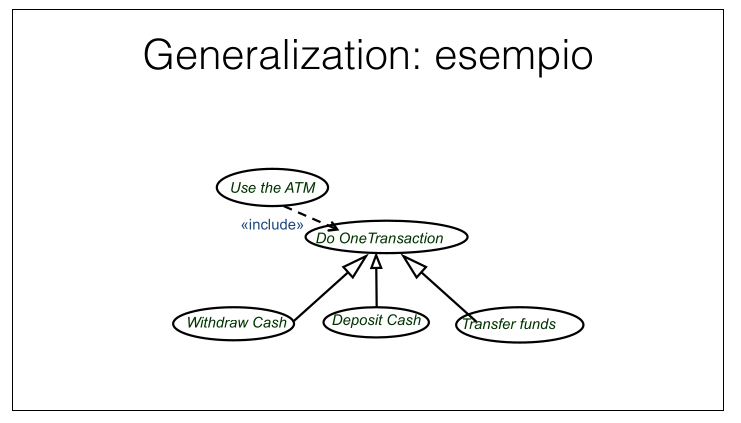
\includegraphics[width=0.75\textwidth]{6}
	\end{center}
	Un caso d'uso base è una generaizzazione di un caso d'uso child, ed è 
	eseguito se la condizione di generalizzaione è vera
	\paragraph{La generalizzazione è fattibile anche sugli attori} esattamente
	come il discorso in java di classi e sottoclassi, uguale
\end{itemize}
\section{Modelli di Dominio}
E' una rappresentazione di classi cncettuali o oggetti del mondo reale di un
dominio. (Non oggetti software), fondamentalmente è l'astrazione visuale della
terminologia e del contenuto informativo del dominio.
\paragraph{Applicando UML} il modello di dominio è un insieme di diagramma delle
classi in cui non sono definite le operazioni MA sono descritte solamente le
classi concettuali, le associazioni tra classi e gli attributi
\paragraph{Esempio:}
\begin{center}
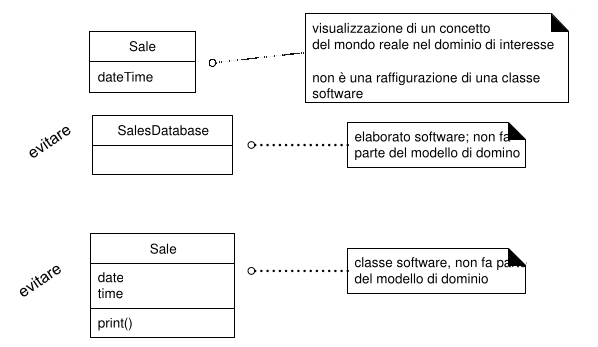
\includegraphics[width=0.75\textwidth]{7}
\end{center}
\paragraph{Ciò che non è un numero o un testo è rappresentato da una classe
contetuale separata}
\subsection{Associazioni}
Un'associazione è una relazione tra classi (prendete Basi di Dati, ecco, mi sto
rincoglionendo anche io con tutti 'sti nomi) e indica una connessione significativa
\begin{center}
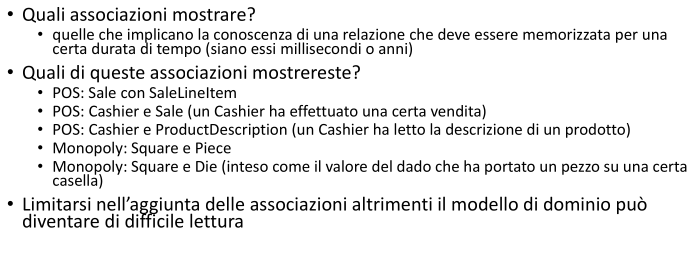
\includegraphics[width=0.75\textwidth]{8}
\end{center}
\subsection{Ruoli}
Il ruolo è l'estremità d un'associazione, può avere molteplicità, nome, 
navigabilità, nei modelli di dominio è usata solo per le molteplicità.
\paragraph{Molteplicità:} Definisce quante istanze di una determinata classe si
possono associare ad un'istanza di un'altra classe
\paragraph{Possibili valori per la Molteplicità: }
\begin{center}
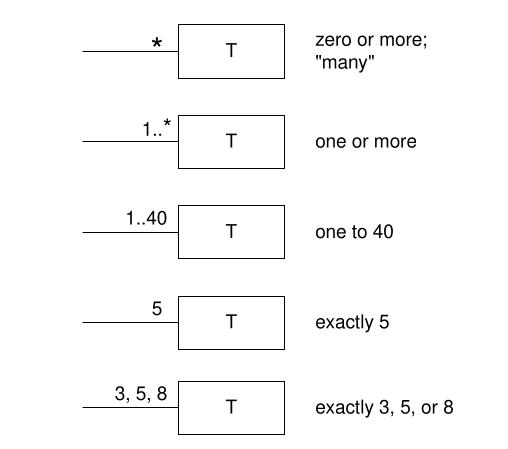
\includegraphics[width=0.75\textwidth]{9}
\end{center}
\paragraph{Notazione per le associazioni:}
\begin{center}
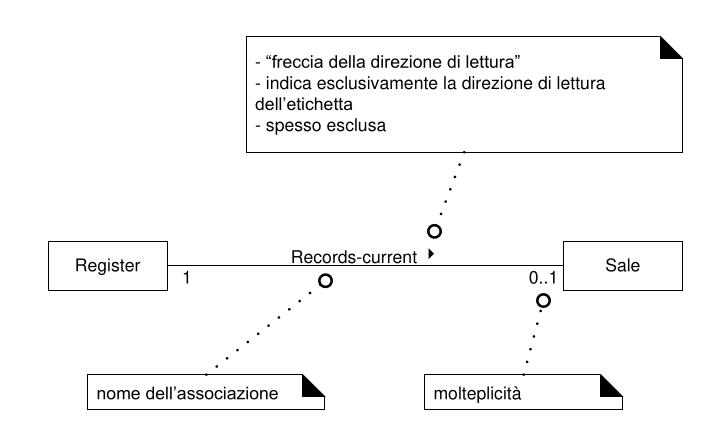
\includegraphics[width=0.75\textwidth]{10}
\end{center}
Si possono fare anche associazioni multiple tra due classi. 
\subsection{Attributi}
Gli attributi sono di tipo primitivo: caratteri, stringhe, numerelli, tipi per
i dati semplici di questo tipo (la stringa anche se è un array di caratteri, 
ormai si considera tipo base). Questi attributi non vanno usati come chiavi esterne.
\section{Contratti delle operazioni di sistema}
Sono una parte dei casi d'uso, ed è un sistema tipo blackbox (pre-condizioni e 
post-condizioni). Un contratto è formato da:
\begin{enumerate}
	\item Operazione
	\item Riferimenti: Casi in cui può verificarsi l'operazione
	\item Pre-Condizioni: Ipotesi sullo stato di sistema PRIMA dell'operazione
	\item Post-Condizioni: Cambiamenti prodotti dall'operazione. Non hanno 
	a che fare necessariamente con il software, potrebbero anche riguardare
	l'hardware.
	\paragraph{Sono descritte dalle seguenti categorie:}
	\begin{enumerate}
		\item Creazione e cancellazione di istanze
		\item Modifica di attributi
		\item Associazioni create oppure eliminate
	\end{enumerate}
\end{enumerate}
\paragraph{Operazione di sistema}
\begin{center}
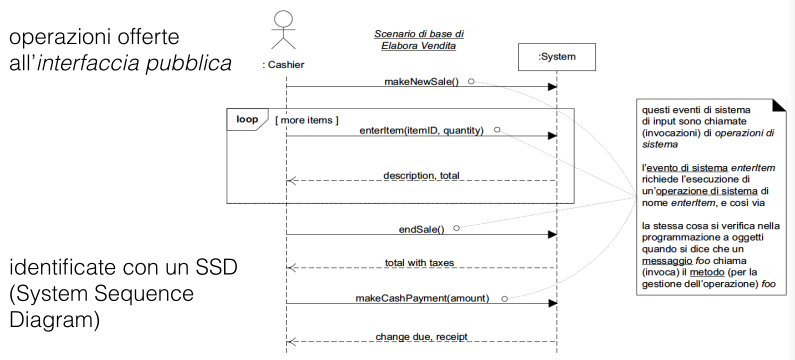
\includegraphics[width=0.75\textwidth]{11}
\end{center}
L'interfaccia publica sarebbe l'insieme delle operazioni del sistema, e comprende
casi d'uso e contratti
\section{Diagrammi di interazione}
\paragraph{Agile Modeling:}
\begin{itemize}
	\item Modellare per comprendere e comunicare
	\begin{itemize}
		\item Modellare insieme agli altri
		\item Creare diversi modelli in parallelo
	\end{itemize}
	\item Modelli dinamici
	\begin{itemize}
		\item Utili per progettare la logica del sistema, il comportamento del codice
		e il corpo dei metodi
		\item Diagrammi di interazione: diagrammi di sequenza e comunicazione 
	\end{itemize}
	\item Modelli statici
	\begin{itemize}
		\item Progettare package, nome delle classi, firme dei metodi, dipendenze
		\item Diagramma dei package, e diagramma delle classi
	\end{itemize}
\end{itemize}
A livello semantico il diagramma di sequenza e comunicazione sono equivalenti,
cambia la notazione,in alcuni casi è più utile applicare uno dei due, in altri
l'altro. Modellano scenari di utilizzo di sistema
\subsection{Diagramma di sequenza}
Si coglie in modo immediato l'ordine in cui vengono scambiati i messaggi. 
L'aspetto temporale è gestito dall'alto verso il basso, quindi in alto le cose
che accadono prima, in baso le ultime, gli oggetti sono tutti posizionati in alto.
\paragraph{Elementi di notazione}
\begin{itemize}
	\item Rettangoli delle Linee di Vita: Rappresentano i partecipanti all'interazione
	dentro ai rettangoli c'è nomeOggetto:nomeClasse, ad esempio Fido:Cane
	\item Sintassi per i messaggi: return = message(parameter:paramtype):returnType
	\paragraph{Esempio:}
	\begin{center}
	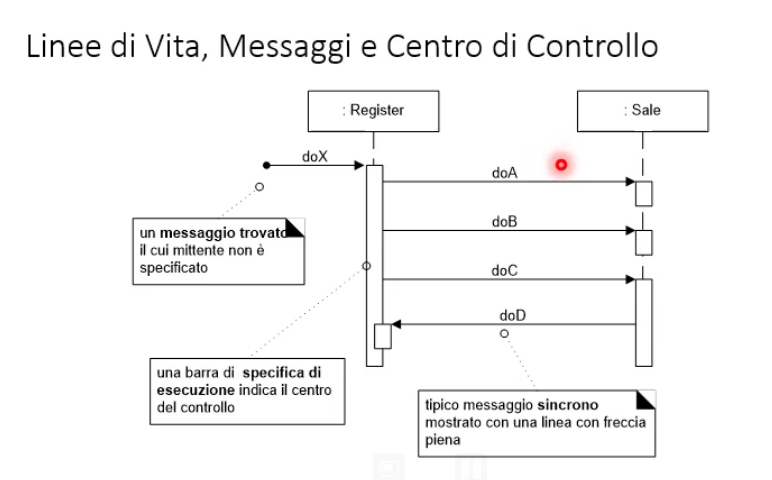
\includegraphics[width=0.75\textwidth]{12}
	\end{center}
	Ps. quel pallino rosso è perchè ho preso dal video, sory
	\item Freccia piena: Messaggio sincrono 
	\item Freccia vuota: Messaggio asincrono, Un esempio di messaggi asincroni
	sono le transazioni
	\item Valori di ritorno: Se lo si vuole indicare si fa una linea tratteggiata
	\item Messaggi a Self: Messaggi inviati a se stessi, riflessivi, ricorsivi
	\item Creazione di istanze: normalmente tutte le istanze si indicano all'inizio,
	se voglio creare una nuova istanza l'oggetto si mette all'altezza di dove viene
	creato
	\item Distruzione di oggetti: Così come si possono creare oggetti possono anche
	distruggersi con il <<destroy>>, e si usa la X alla fine della freccia
	\item Frames: Sono dei rettangoli in cui ci sono dei messaggi che sono relativi
	al frame indicato
	\paragraph{A che serve?} \begin{center}
	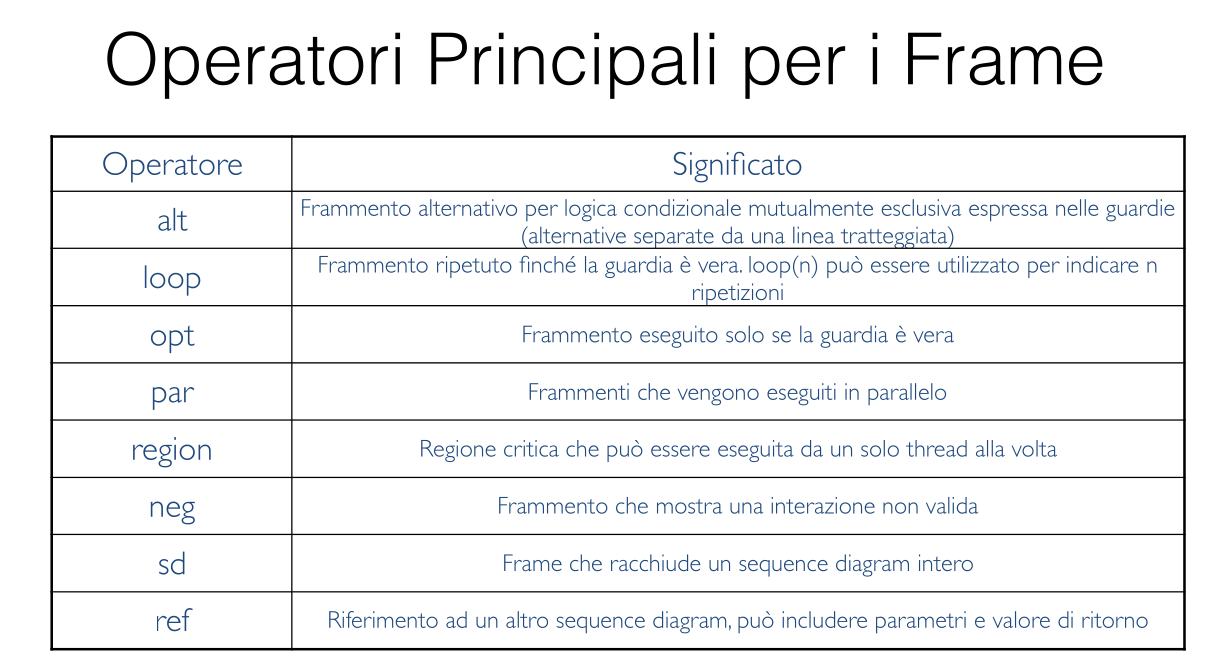
\includegraphics[width=0.75\textwidth]{13}
	\end{center}
	\begin{itemize}
		\item Frame alt: 
		\begin{center}
		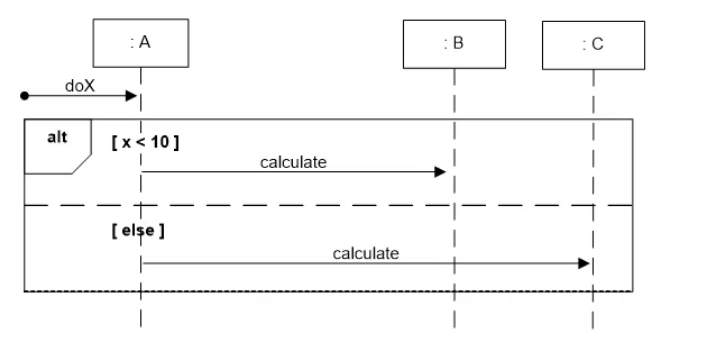
\includegraphics[width=0.75\textwidth]{14}
		\end{center}
		Alt indica un'alternativa, sopra hai una condizione, sotto l'altra e poi
		hai in mezzo la linea tratteggiata
		\item Frame loop:
		\begin{center}
		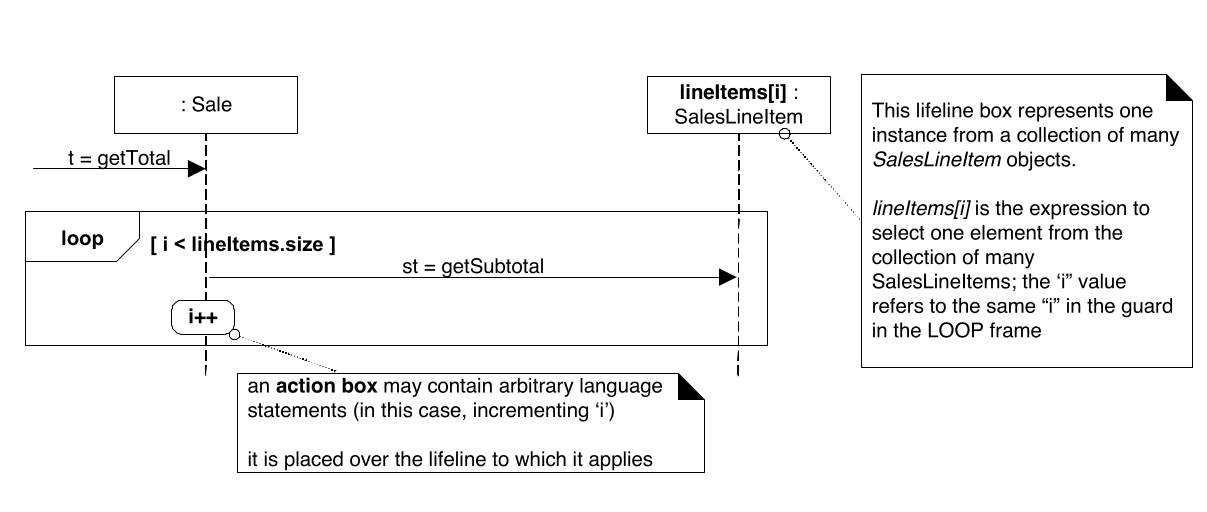
\includegraphics[width=0.75\textwidth]{15}
		\end{center}
		Anche qua hai la condizione booleana, ma serve per loopare e non per fare
		if
		\item Frame opt:
		\begin{center}
		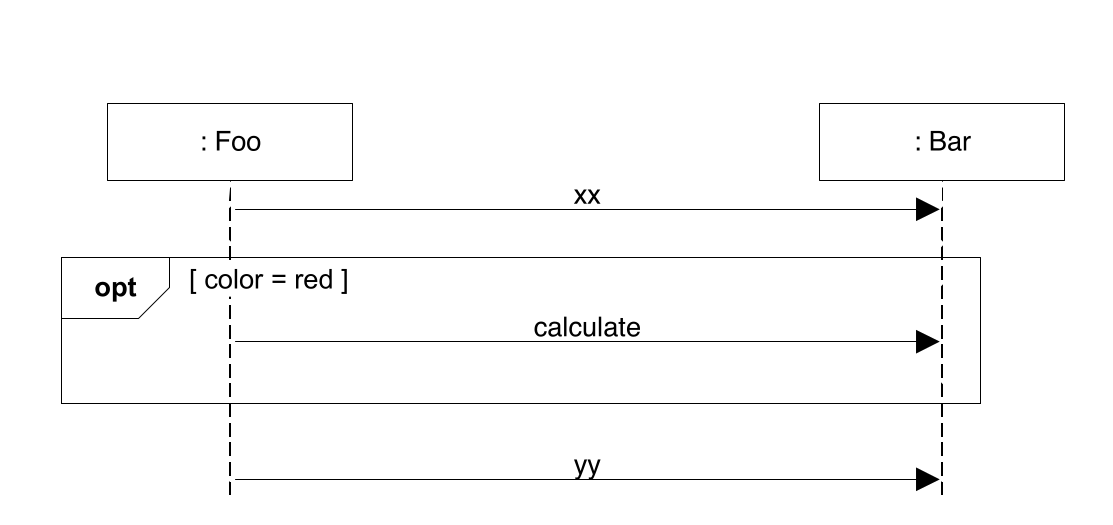
\includegraphics[width=0.75\textwidth]{16}
		\end{center}
		Opzionale, una booleana, se è vero allora fai, altrimenti niente, come
		l'if senza else
		\item Frame par:
		\begin{center}
		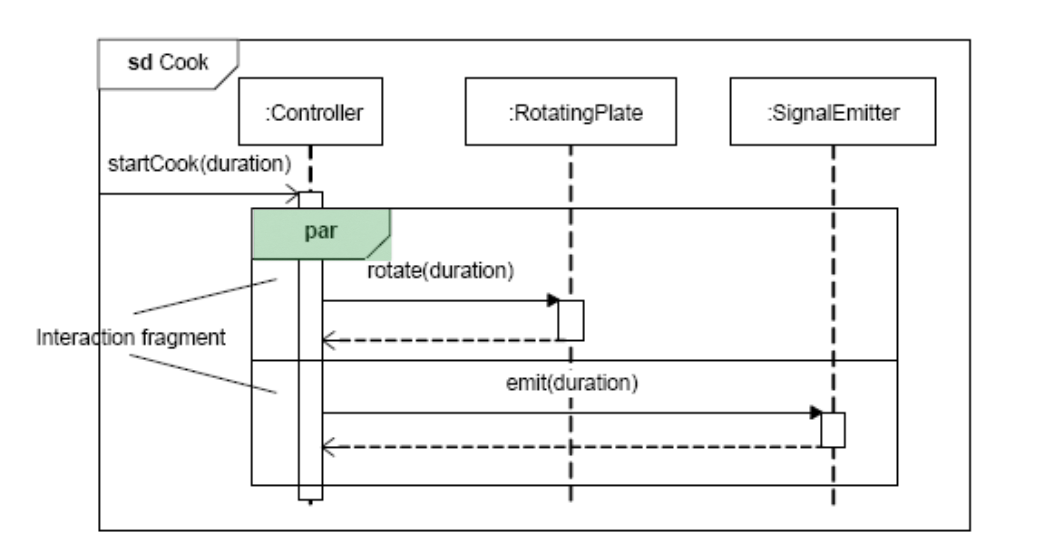
\includegraphics[width=0.75\textwidth]{17}
		\end{center}
		Parallelo, due sequenze di messaggi in parallelo.. eeeasy
		\item Frame region:
		\begin{center}
		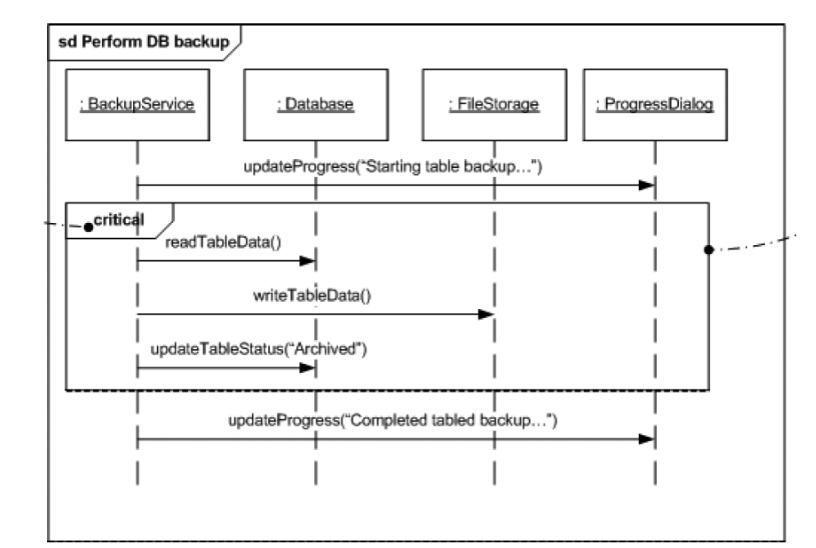
\includegraphics[width=0.75\textwidth]{18}
		\end{center}
		Indica una regione critica che si affida ad un solo thread
		\item Frame neg:
		\begin{center}
		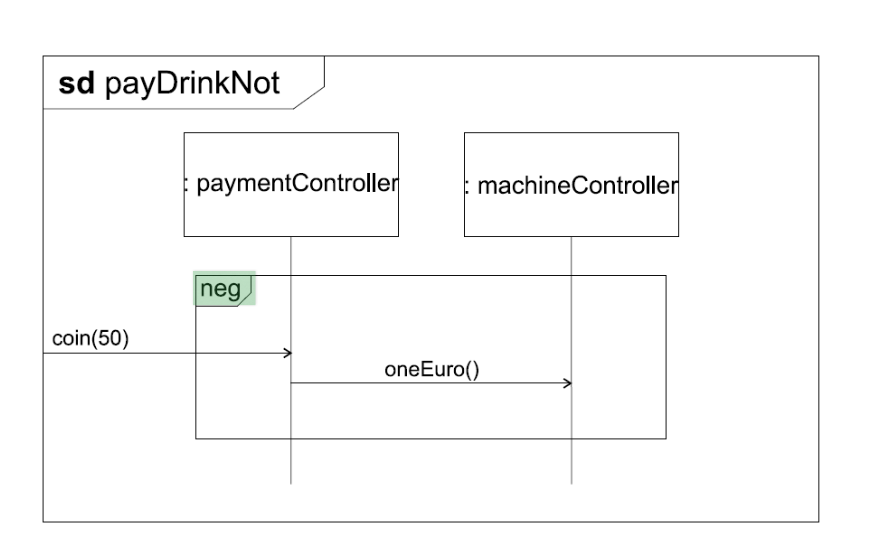
\includegraphics[width=0.75\textwidth]{19}
		\end{center}
		Indica qualcosa che non è permesso, da esempio se metto 50 cent, ho neg
		su un'euro
		\item Frame sd:
		\begin{center}
		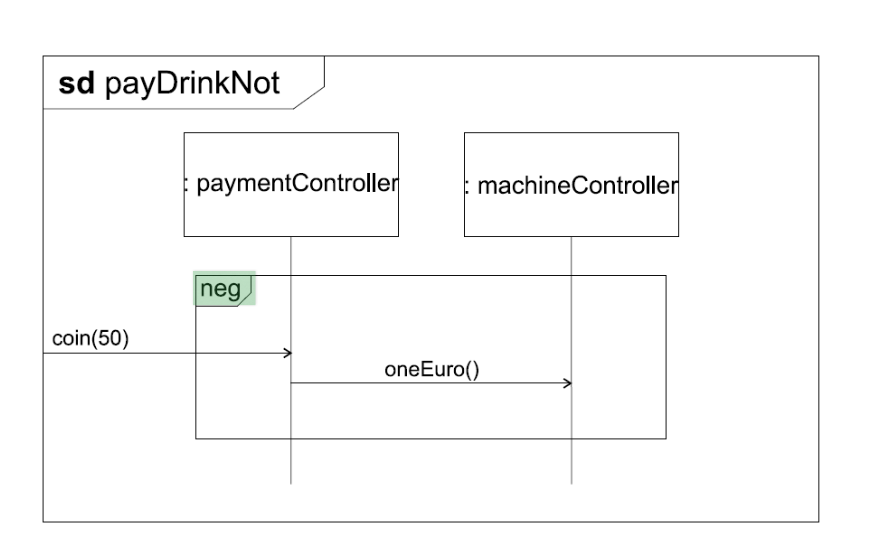
\includegraphics[width=0.75\textwidth]{19}
		\end{center}
		\item Frame ref:
		\begin{center}
		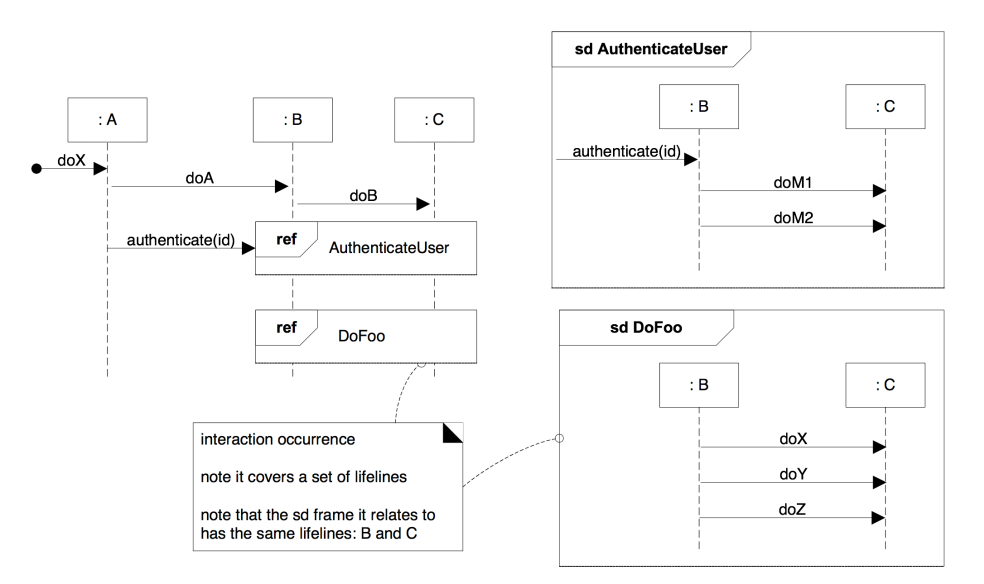
\includegraphics[width=0.75\textwidth]{20}
		\end{center}
		Quando un diagramma diventa troppo grande e difficile da leggere, si può
		tirare fuori un diagramma e mettere da parte il riferimento
		\item Frame annidato:
		\begin{center}
		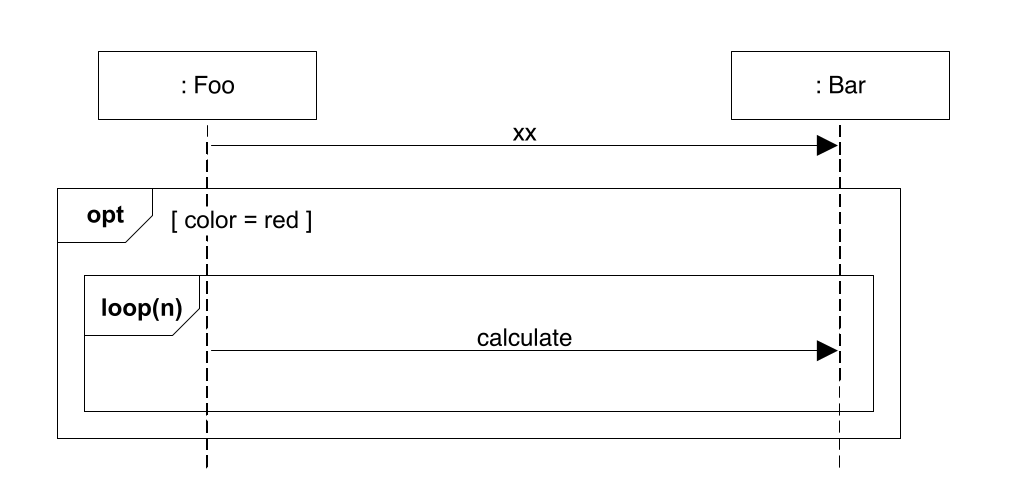
\includegraphics[width=0.75\textwidth]{21}
		\end{center}
		Si possono innestare i frame
	\end{itemize}
	\item Invocazione di metodi statici
	\item Chiamate polimorfe
	\item Chiamate asincrone e oggetti attivi: non tantissimo usate ma potrebbero
	capitare
\end{itemize}
\subsection{Diagramma di comunicazione}
Semanticamente identico al Diagramma di sequenza,
\paragraph{Elementi di notazione}
\begin{itemize}
	\item Collegamenti: Un collegamento è un percorso di connessione tra due
	oggetti, e indica la forma di navigazione e visibilità
	\item Messaggi: Si usano numeri di sequenza per mostrare l'ordine sequenziale
	dei messaggi (Nel thread di controllo corrente)
	\item Messaggi a self
	\item Creazione di un'istanza: Non c'è il problema di creare gli oggetti
	tutti in alto come nei diagrammi di sequenza
	\item Sequenza complessa: Non si ha facilità di comprensione dell'ordine
	in cui sono inviati i messaggi
	\item Messaggi condizionali: Viene inviato solo se la sua guardia (o condizione)
	è vera
	\item Percorsi mutualmente esclusivi: Sono condizioni booleane con il ! davanti
	\item Iterazioni o cicli: Si possono formare dei cicli, delle iterazioni, 
	nei diagrammi di sequenza questi erano i frame
	\item Invocazione di un metodo statico 
	\item Messaggi polimorfi: Questa è identica al diagramma di sequenza, con 
	RSA si può generare l'uno a partire dall'altro indipendentemente
	\item Chiamate Asincrone: Anche qua c'è il clock come oggetto attivo, stesso
	identico concetto di prima
\end{itemize}
\end{document}